\documentclass[12pt,letterpaper]{article}

\newenvironment{proof}{\noindent{\bf Proof:}}{\qed\bigskip}

\newtheorem{theorem}{Theorem}
\newtheorem{corollary}{Corollary}
\newtheorem{lemma}{Lemma} 
\newtheorem{claim}{Claim}
\newtheorem{fact}{Fact}
\newtheorem{definition}{Definition}
\newtheorem{assumption}{Assumption}
\newtheorem{observation}{Observation}
\newtheorem{example}{Example}
\newcommand{\qed}{\rule{7pt}{7pt}}

\newcommand{\assignment}[4]{
\thispagestyle{plain} 
\newpage
\setcounter{page}{1}
\noindent
\begin{center}
\framebox{ \vbox{ \hbox to 6.28in
{\bf CS446: Machine Learning \hfill #1}
\vspace{4mm}
\hbox to 6.28in
{\hspace{2.5in}\large\mbox{Problem Set #2}}
\vspace{4mm}
\hbox to 6.28in
{{\it Handed Out: #3 \hfill Due: #4}}
}}
\end{center}
}

\newcommand{\solution}[4]{
\thispagestyle{plain} 
\newpage
\setcounter{page}{1}
\noindent
\begin{center}
\framebox{ \vbox{ \hbox to 6.28in
{\bf CS446: Machine Learning \hfill #4}
\vspace{4mm}
\hbox to 6.28in
{\hspace{2.5in}\large\mbox{Problem Set #3}}
\vspace{4mm}
\hbox to 6.28in
{#1 \hfill {\it Handed In: #2}}
}}
\end{center}
\markright{#1}
}

\newenvironment{algorithm}
{\begin{center}
\begin{tabular}{|l|}
\hline
\begin{minipage}{1in}
\begin{tabbing}
\quad\=\qquad\=\qquad\=\qquad\=\qquad\=\qquad\=\qquad\=\kill}
{\end{tabbing}
\end{minipage} \\
\hline
\end{tabular}
\end{center}}

\def\Comment#1{\textsf{\textsl{$\langle\!\langle$#1\/$\rangle\!\rangle$}}}


\usepackage{amsmath,amssymb,url,color,multirow,array,graphicx}
\sloppy
\newcommand{\ignore}[1]{}
\oddsidemargin 0in
\evensidemargin 0in
\textwidth 6.5in
\topmargin -0.5in
\textheight 9.0in

\begin{document}

\solution{Chen Zhang}{10/11/2014}{3}{Fall 2014}
% Fill in the above, for example, as follows:
% \solution{Joe Smith}{\today}{1}{Fall 2012}

\pagestyle{myheadings}  % Leave this command alone

\section{Problem 1}
In this problem, I implemented my code as required. I looped over all the parameter combinations and tuned the learning algorithm, and found best parameters and use them in the training process. The main result is the Table. 1 and Fig. 1 and Fig. 2. Depending on different l m n combination, the best parameter after tuning is also different. 

\noindent From Fig.1 we can see that when $n=500$, algorithms with margin behaves better than cases without margin( perceptron and winnow). But the advantage is not very obvious. Ada Grad, Winnow, Winnow with margin have a better behavior on the number of mistakes it make as number of example increases. These three algorithms tend to converge to a certain value, while perceptron and perceptron with margin does not have a very clear convergence to some value. 

\noindent When $n=1000$, we can see that the margin does not have a obvious effect on the behavior of the algorithms. The number of mistakes all the algorithms make are larger than the case of $n=500$. But the convergence property of winnow, winnow with margin and ada grad still holds, while perceptron and perceptron still does not have a clear convergence. 
\begin{center}
	\begin{table}[!hbp]
		\begin{tabular}{|p{4.3cm}<{\centering}|p{2.5cm}<{\centering}|p{4cm}<{\centering}|p{4cm}<{\centering}|}
			\hline
			\multirow{2}{*}{Algorithm} & \multirow{2}{*}{Parameters} & \multicolumn{2}{|c|}{Data Set} \\
			\cline{3-4}
			& & $n=500$& $n=1000$\\
			\hline
			%Perceptron    & $\eta$               &                             &                                   \\\hline \hline
			Perceptron w/margin &          $\eta$          &     0.03              &               0.005                \\ \hline
			%\cline{2-4}
			%& $\gamma$ &  & \\ \hline \hline
			Winnow               &     $\alpha$           &         1.1            &         1.1                          \\\hline %\hline
			\multirow{2}{*}{Winnow w/margin}     & $\alpha$&      1.1                           &             1.1        \\
			\cline{2-4}
			& $\gamma$ & 2 & 0.006 \\ \hline %\hline
			AdaGrad             & $\eta$&              0.25                        &             0.25                      \\\hline %\hline
			%\multirow{2}{*}{AdaGrad w/margin}    & $\eta$&                                               &                                   \\
			%      \cline{2-4}
			%      & $\gamma$ &  & \\ \hline
		\end{tabular}
			\caption{Problem 1 Table for the best Parameters}
	\end{table}
\end{center}

\begin{figure}[h!]
	\centering
	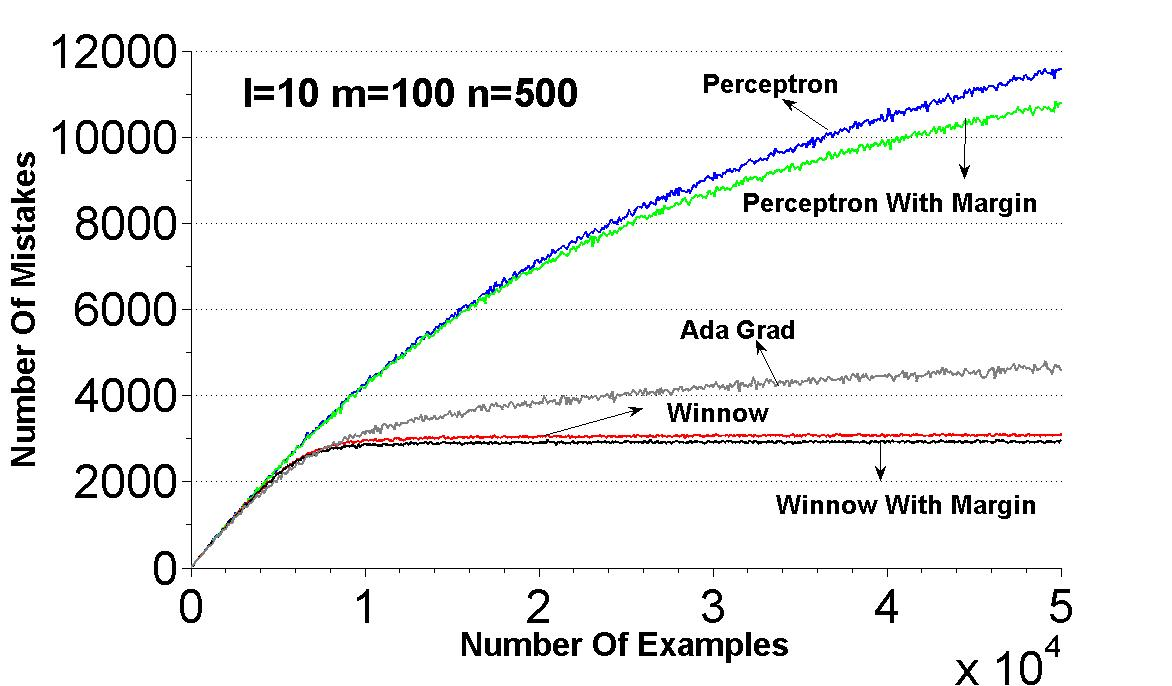
\includegraphics[width=1\textwidth]{Problem1Figure1}
	\caption{First Figure of Problem 1}
\end{figure}

\begin{figure}[h!]
	\centering
	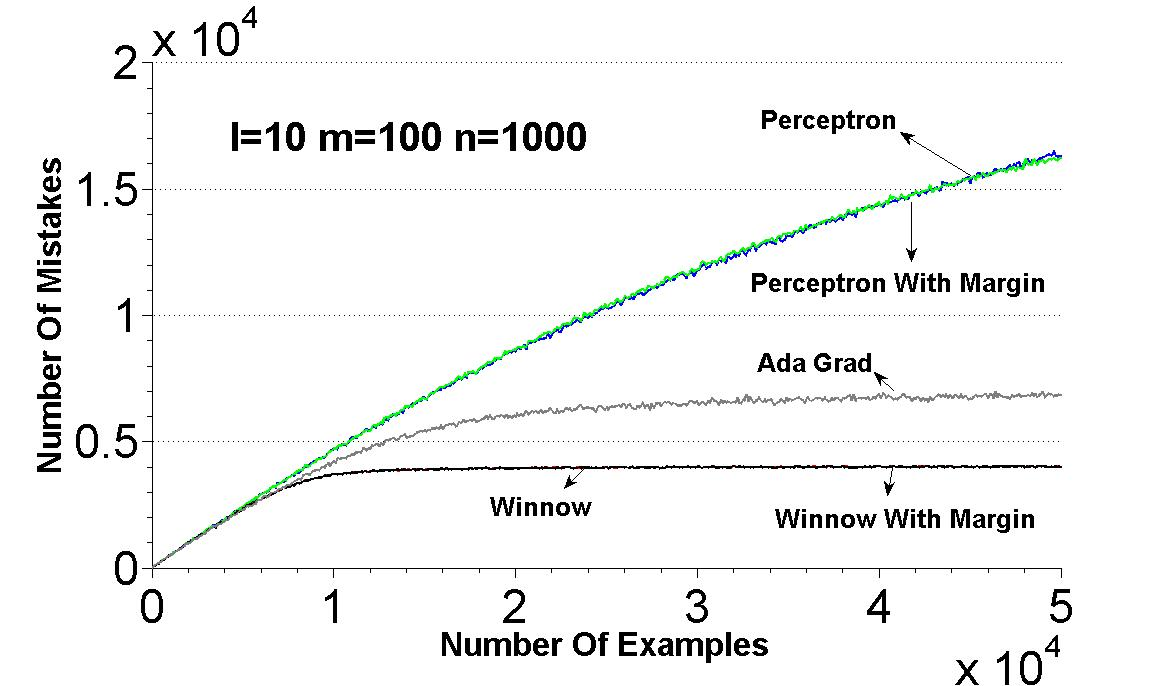
\includegraphics[width=1\textwidth]{Problem1Figure2}
	\caption{Second Figure of Problem 2}
\end{figure}

\section{Problem 2}
In this problem, I implemented my code as required. I looped over all the parameter combinations and tuned the learning algorithm, and found best parameters and use them in the training process, as is shown in Table. 2. I then used $R=1000$ to calculate the number of mistakes it made before reaching the criteria. 

\noindent From Fig. 3 we can see that winnow and winnow with margin has the best behavior. Perceptron has the largest number of mistakes before reaching the criteria. Perceptron with margin has better behavior than ada grad when n is small but worse behavior when n is large. Similar to the Fig. 1 and Fig. 2, winnow and winnow with margin also have a convergence trend, while the other three algorithms does not have a clear convergence evident. 

\begin{table}[!hbp]
	\begin{tabular}{|p{4.7cm}<{\centering}|p{2.0cm}<{\centering}|p{1.5cm}<{\centering}|p{1.5cm}<{\centering}|p{1.5cm}<{\centering}|p{1.5cm}<{\centering}|p{1.5cm}<{\centering}|}
		\hline
		\multirow{2}{*}{Algorithm} & \multirow{2}{*}{Parameters} & \multicolumn{5}{|c|}{Data Set} \\
		\cline{3-7}
		& & $n=40$& $n=80$& $n=120$& $n=160$& $n=200$\\
		\hline
		% Perceptron    & $\eta$               &                             &   & & &                              \\\hline \hline
		Perceptron w/margin &          $\eta$          &       1.5            &  0.25   & 0.03 & 0.03 &       0.03                       \\\hline
		
		%& $\gamma$ &  & & & &\\ \hline \hline
		Winnow               &     $\alpha$           &      1.1               &     1.1    & 1.1 & 1.1 &        1.1                  \\\hline %\hline
		\multirow{2}{*}{Winnow w/margin}     &  $\alpha$&              1.1                       & 1.1    & 1.1 & 1.1 &         1.1       \\
		\cline{2-7}
		& $\gamma$ &  2 &  2 & 0.3 & 2 & 2 \\ \hline %\hline
		AdaGrad             &  $\eta$&                      1.5                &  1.5             & 1.5& 1.5&       1.5             \\\hline %\hline
		%\multirow{2}{*}{AdaGrad w/margin}    & $\eta$&                                               &   & & &                                \\
		%      \cline{2-7}
		%      & $\gamma$ &  & & & &\\ \hline
	\end{tabular}
	\caption{Problem 2 Table for the best Parameters}
\end{table}

\section{Problem 3}
In this problem, I implemented my code as required. I generated data with noise and looped over all the parameter combinations and tuned the learning algorithm, and found best parameters and use them in the training process, as is shown in Table. 3. In the table, we could see that perceptron with margin and ada grad tend to behave the best, while in the problem 2, winnow and winnow with margin tend to behave best. This shows than when the data has noise, linear increment with margin would be the best algorithm to solve the problem
\begin{center}
	\begin{table}
		\begin{tabular}{|p{4.3cm}<{\centering}|p{2.5cm}<{\centering}|p{2.7cm}<{\centering}|p{2.7cm}<{\centering}|p{2.7cm}<{\centering}|}
			\hline
			\multirow{2}{*}{Algorithm} & \multirow{2}{*}{Parm \& Accy} & \multicolumn{3}{|c|}{Data Set} \\
			\cline{3-5}
			& & $m=100$& $m=500$& $m=1000$\\
			\hline
			Perceptron    & Accy \%               &            91.19                 &  88.99 &             64.01                  \\ \hline
			%      \cline{2-5}
			%      & Accy\% &  & & \\ \hline \hline
			\multirow{2}{*}{Perceptron w/margin} &          $\eta$          &         0.03          &    1.5 &            0.25                   \\
			\cline{2-5}
			%& $\gamma$ &  & & \\
			%\cline{2-5}
			& Accy\% &  98.34& 88.99& 64.8\\ \hline \hline
			\multirow{2}{*}{Winnow}               &     $\alpha$           &      1.1               &     1.1    &         1.1                  \\
			\cline{2-5}
			& Accy\% &  91.62& 84.76 & 69.37\\ \hline \hline
			\multirow{3}{*}{Winnow w/margin}     & $\alpha$&             1.1                        &    1.1 &   1.1             \\
			\cline{2-5}
			& $\gamma$ &  0.006& 0.3& 0.04\\
			\cline{2-5}
			& Accy\% &  96.54& 88.74& 69.9\\ \hline \hline
			\multirow{2}{*}{AdaGrad}             & $\eta$&                 0.25                     &       0.25        &     1.5                \\
			\cline{2-5}
			& Accy\% &  99.96& 96.78& 76.05\\ \hline %\hline
			%\multirow{3}{*}{AdaGrad w/margin}    & $\eta$&                                               &   &                                \\
			%      \cline{2-5}
			%      & $\gamma$ &  & &\\
			%      \cline{2-5}
			%      & Accy\% &  & & \\\hline
		\end{tabular}
			\caption{Problem 3 Table for the best Parameters}
	\end{table}
\end{center}

\begin{figure}[h!]
	\centering
	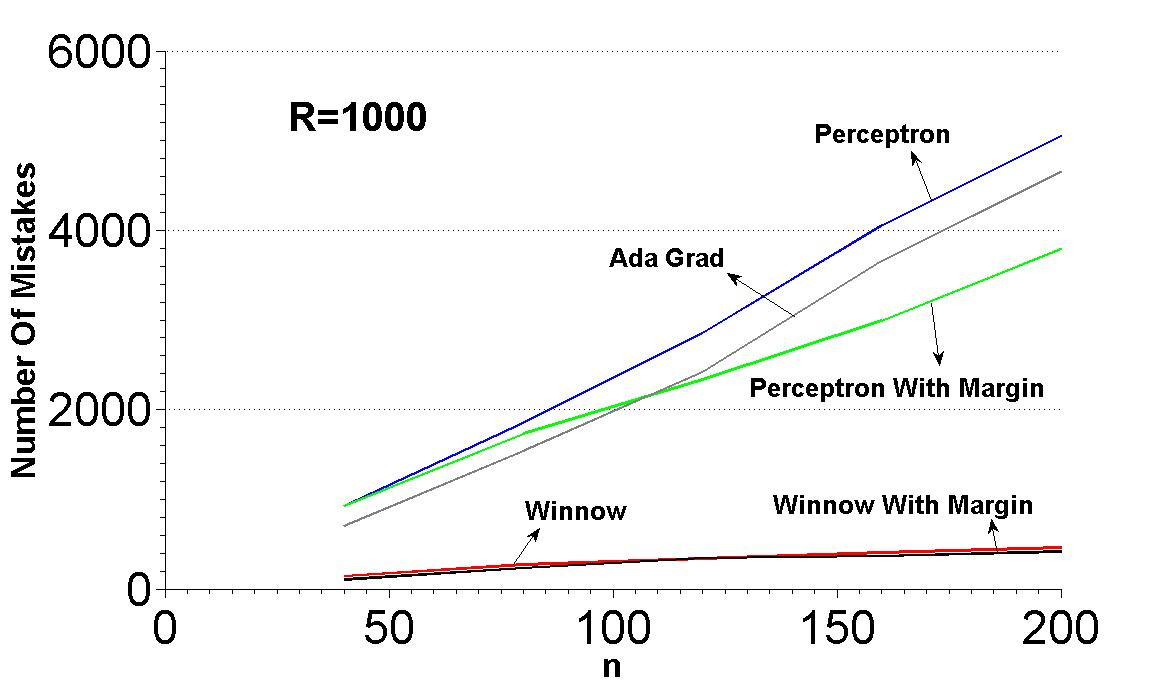
\includegraphics[width=1\textwidth]{Problem2Figure1}
	\caption{First Figure of Problem 2}
\end{figure}

\section{Bonus Problem}
In this problem, I implemented my code as required. I generated unbalanced data, use perceptron for the three cases to calculate the accuracy. Then I tuned perceptron with margin, and used the best case to calculate the accuracy on the unbalanced data. The result is shown in the Table. 4. 

\noindent We see that perceptron and perceptron with margin has extremely good behavior on the unbalanced data set. This shows that perceptron has extremely robust behavior on linearly separable data set. 
\begin{center}
	\begin{table}
		\begin{tabular}{|p{4.3cm}<{\centering}|p{2.5cm}<{\centering}|p{2.7cm}<{\centering}|p{2.7cm}<{\centering}|p{2.7cm}<{\centering}|}
			\hline
			\multirow{2}{*}{Algorithm} & \multirow{2}{*}{Parm \& Accy} & \multicolumn{3}{|c|}{Data Set} \\
			\cline{3-5}
			& & $m=100$& $m=500$& $m=1000$\\
			\hline
			Perceptron    & Accy \%               &            99.85                 &  99.79 &             99.98                  \\ \hline
			%      \cline{2-5}
			%      & Accy\% &  & & \\ \hline \hline
			\multirow{2}{*}{Perceptron w/margin} &          $\eta$          &         0.03          &    0.03 &            0.03                   \\
			\cline{2-5}
			%& $\gamma$ &  & & \\
			%\cline{2-5}
			& Accy\% &  99.53& 99.98& 100\\ \hline %\hline
 %\hline
			%\multirow{3}{*}{AdaGrad w/margin}    & $\eta$&                                               &   &                                \\
			%      \cline{2-5}
			%      & $\gamma$ &  & &\\
			%      \cline{2-5}
			%      & Accy\% &  & & \\\hline
		\end{tabular}
			\caption{Bonus Problem Table for the best Parameters}
	\end{table}
\end{center}

\end{document}

